\documentclass[12pt,a4paper,openany]{book}
\usepackage{lmodern}
\usepackage[svgnames]{xcolor} % Required to specify font color
\input{../LaTexTemplate/templates/couleurs.tex}

\usepackage{makeidx}
\usepackage[utf8]{inputenc} 
\usepackage{marvosym}
\usepackage[T1]{fontenc}
\usepackage[francais]{babel}
\usepackage[top=1.7cm, bottom=1.7cm, left=1.7cm, right=1.7cm]{geometry}
\usepackage{verbatim}
\usepackage[urlbordercolor={1 1 1}, linkbordercolor={1 1 1}, linkcolor=vert1, urlcolor=bleu, colorlinks=true]{hyperref}
\usepackage{tikz} %Vectoriel
\usepackage{listings}
\usepackage{fancyhdr}
\usepackage{multido}
\usepackage{amssymb}
\usepackage{slashbox}
\usepackage{float}
\usepackage[francais]{minitoc}
\usepackage[final]{pdfpages} 
\usepackage{pgfgantt}
\usepackage{graphicx} % Required for box manipulation
\usepackage{makeidx}
\usepackage{lscape}
\usepackage{rotating}
\usepackage{epstopdf}


\newcommand{\titre}{Maison Intelligente}
%\newcommand{\logoFooter}{\begin{minipage}{0.1\textwidth}\includegraphics[width=2cm]{../../images/FACT_official.png}\end{minipage}}
\newcommand{\titreFooter}{Maison Intelligente} 
\newcommand{\subtitle}{Salle de bain} 
\newcommand{\auteur}{}
\newcommand{\semestre}{}
\newcommand{\annee}{2016}


\newcommand{\pole}{}
\newcommand{\sigle}{}
\newcommand{\FactDev}{\textit{FactDev}}
\newcommand{\key}[1]{\textit{#1}}
\newcommand{\approved}{true}

\makeindex
\usepackage[totoc]{idxlayout}


\input{../LaTexTemplate/templates/listings.tex}
\input{../LaTexTemplate/templates/classroomsTemplates/l3/cours.tex}
\input{../LaTexTemplate/templates/remarquesExempleAttention.tex}
\input{../LaTexTemplate/templates/polices.tex}
\input{../LaTexTemplate/templates/affichageChapitre.tex}

\input{../LaTexTemplate/templates/cover/couverture.tex}
\makeatother
\includeonly {
	contents/0_introduction,
	contents/1_diagram_exigences,
	contents/2_diagram_use_case,
	contents/3_diagram_blocks_bdd,
	contents/4_diagram_blocks_ibd,
	contents/5_diagram_states,
	contents/6_diagram_sequences
}
\begin{document}
	\thispagestyle{empty} % Removes page numbers
%	\titleBC
	\dominitoc
	\setcounter{tocdepth}{1}
	\setcounter{secnumdepth}{3}
	\setcounter{minitocdepth}{1}
	
	\tableofcontents

	% Introcution #1 -----------------------
	\chapter*{À propos}

La \textbf{Maison Intelligente} (MI) constitue un lieu où technologies et sciences humaines se rencontrent pour trouver des solutions permettant d'aider à l'accompagnement du vieillissement des populations dans notre société (handicaps, dépendances, etc).
 
Pour ce faire, la Maison Intelligente propose un ensemble de solutions permettant à celle-ci de s'adapter à son habitant.  L'ensemble des possibilités qu'offre la MI sont définies dans le document : M2DL2015-ExigencesMI.
% (cf. https://docs.google.com/spreadsheets/d/1-yaW8fZHG9i6r7vJ7NOU9-66-hnDYY66Vd9cmZTYs2A/edit ). 


L'objectif du document est de proposer un ensemble de diagrammes définies au moyen de la norme SysML répondant aux exigences relatives à la \textbf{salle de bain} de la MI.

Les diagrammes ici représentés seront :
\begin{itemize}
	\item diagramme des \textbf{exigences} (req)
	\item diagramme des \textbf{cas d'utilisation} (uc)
	\item diagramme de \textbf{blocs de définition} (bdd)
	\item diagramme \textbf{interne de blocs} (idb)
	\item diagramme comportementaux
	\begin{itemize}
		\item diagramme d'\textbf{états} (st)
		\item diagramme de \textbf{séquences} (seq)
	\end{itemize}
\end{itemize} 		
	
	\chapter{Diagramme des exigences (req)}
 % Diagramme des exigences #2	
	\chapter{Diagramme des cas d'utilisations}
  % Diagramme des cas d'utilisation #3
\chapter{Diagrammes de blocs de définition}
\section{Diagramme de blocs général}
Afin de répondre à l'ensemble des exigences présentées section \ref{req}, figure \ref{fig:requirements}, la salle de bain possède différents blocs : 
\begin{description}
	\item[Mobilier] Concerne les équipements devant s'adapter à l'habitant
	\item[Éclairages] Tout ce qui est prévu pour l'adaptation des éclairages
	\item[Radiateur] L'adaptation de la température de la pièce
	\item[Contrôleur] Un système permettant de contrôler les éléments de notre salle de bain. Ce système contient un micro-contrôleur permettant l'utilisation des capteurs et actionneurs, un système de communication avec les données de la maison intelligente, ainsi qu'un logiciel effectuant les traitements nécessaires (monter/descendre un mobilier, augmenter la température de la pièce, \ldots)
\end{description}
\vfill

\begin{figure}[H]
	\hspace{-40px}
	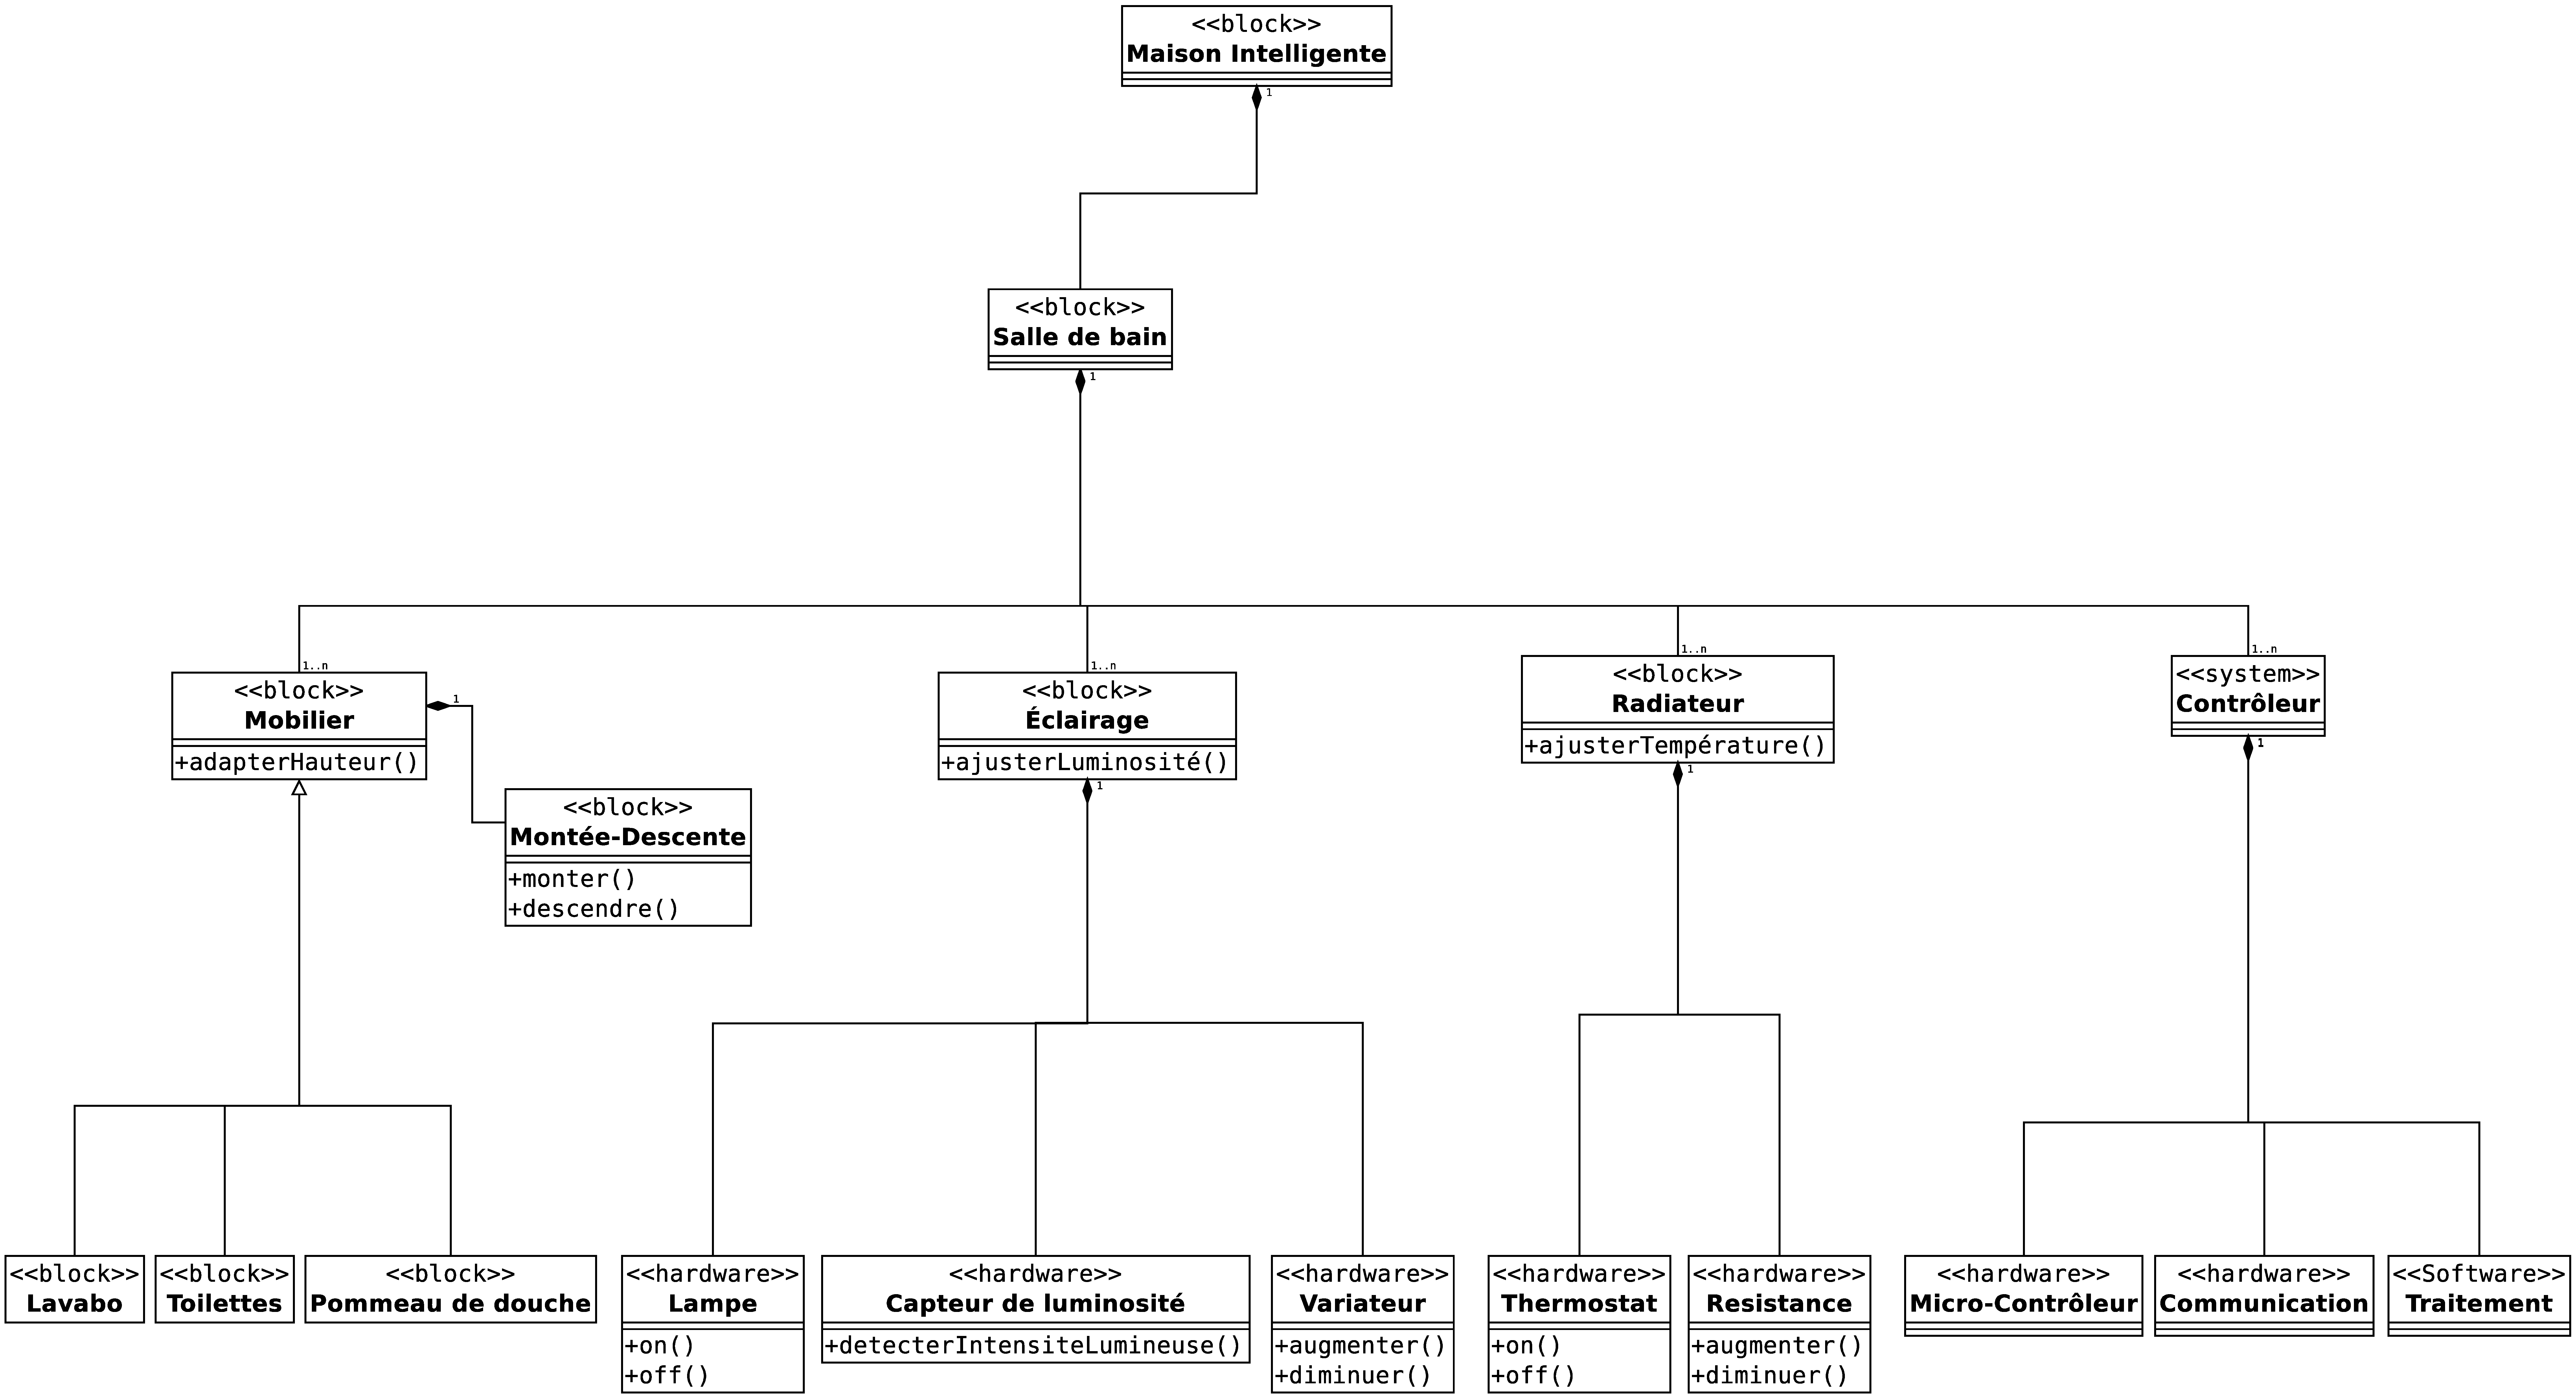
\includegraphics[width=1.16\linewidth]{diagrams/bathroom/diagramme_blocks_bdd.eps}
	\caption{Diagramme de blocs de définition « général »}
	\label{fig:diagramme_bdd}
\end{figure}
\vfill
\pagebreak
\section{Diagramme de blocs de « Montée-Descente »}
Chaque mobilier doit pouvoir moduler sa hauteur pour s'adapter à l'habitant de la MI. Chaque mobilier de la salle de bain est doté d'un bloc « Montée-Descente » comportant :
\begin{description}
	\item[Capteur de mouvement Infra-Rouge] détermine les mouvements de l'habitant
	\item[Capteur laser] permet de déterminer la taille de l'habitant afin de pouvoir s'adapter à lui (montée-descente des meubles)
	\item[Système élévateur] permet de monter ou descendre la dalle supportant le mobilier (ou l'habitant si celui-ci est dans la douche) en fonction de sa position actuelle et de la taille de l'habitant.   
\end{description}
\vfill
\begin{figure}[H]
	\centering
	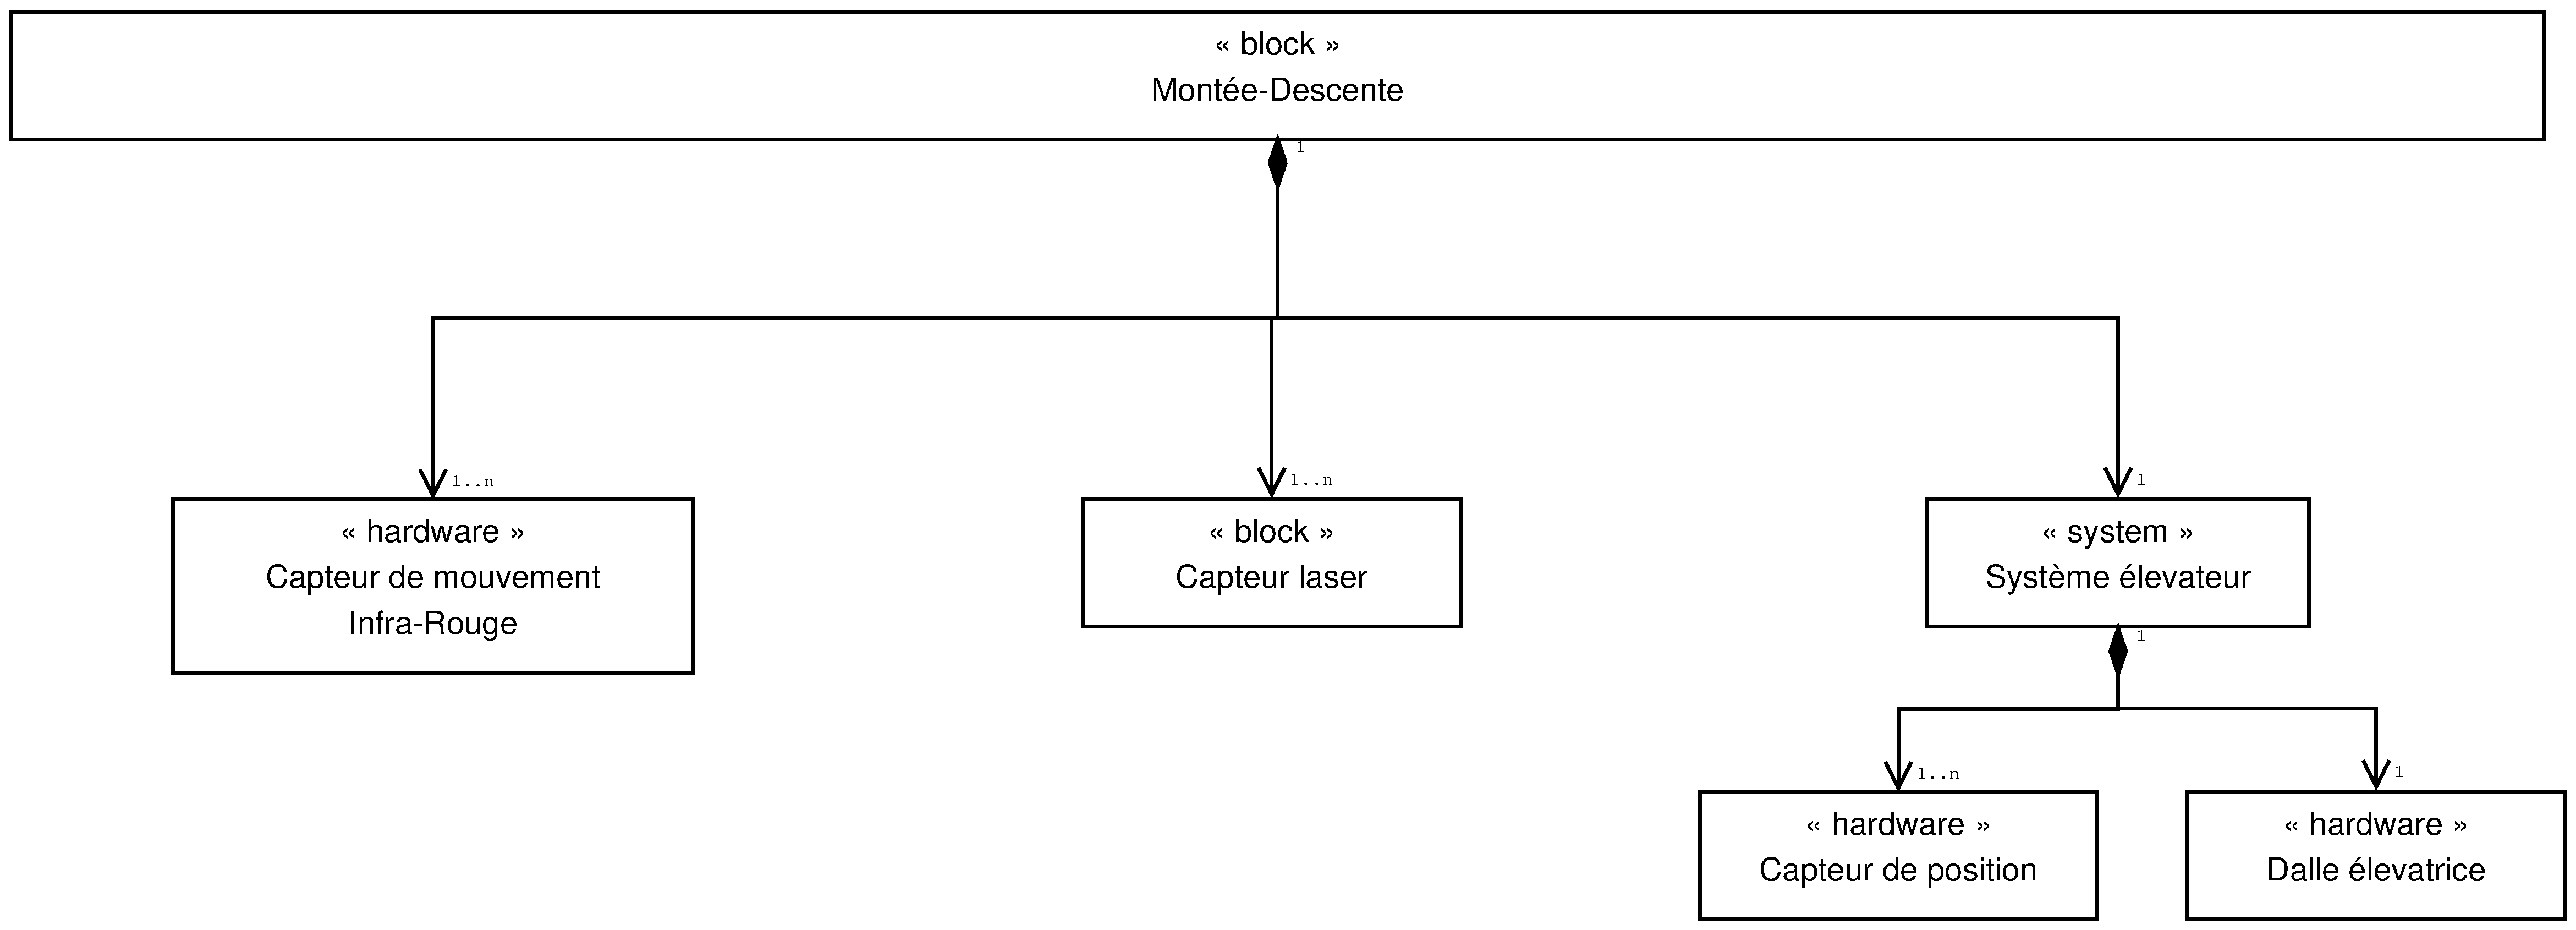
\includegraphics[width=1.0\linewidth]{diagrams/bathroom/diagramme_blocks_bdd2.eps}
	\caption{Diagramme de blocs de définition de « Montée-Descente »}
	\label{fig:diagramme_bdd2}
\end{figure}
\vfill
 % Diagrammes de blocks (bdd) #4	
	\chapter{Diagrammes internes de blocks (ibd)}
 % Diagrammes de blocks (ibd) #5
	% Diagrammes comportementaux
	\section{Diagrammes d'états (st)}
TODO	% diagramme d'états (st) #6		
	\section{Diagrammes de séquences}	% diagrammes de séquences #7	

%	\include{contents/references}
	
	\listoffigures
	\printindex

\enddocument}
